
% \subsection{Learning Management System}
At UNLaM, the Microsoft Teams platform was used to replace classroom interaction with students with videoconferencing during the SARS-CoV-2 lockdowns.
After each meeting its recording was published to a different page, or channels in the system's terminology, as shown at the left at the figure \ref{fig:teams}.

\begin{figure}[!ht]
\centering
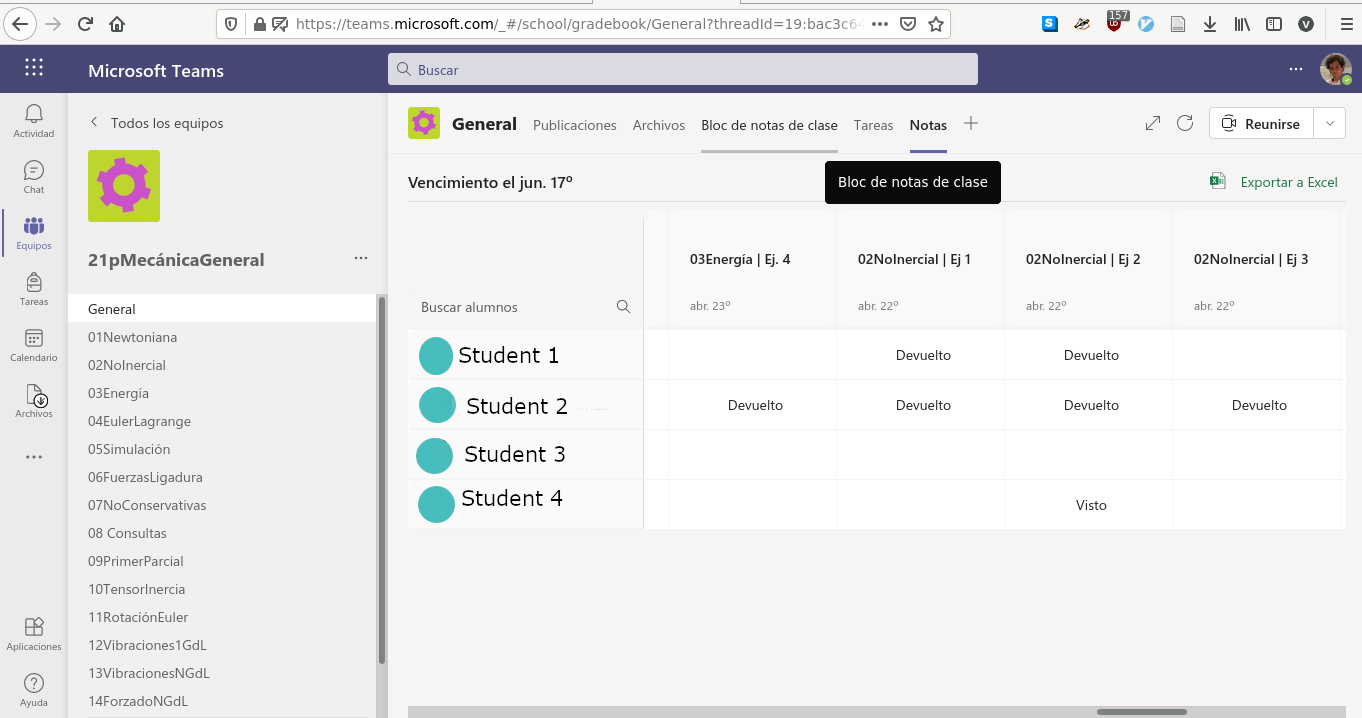
\includegraphics[width=\linewidth]{figuras/notasTeams2.png}
\caption{Separate channels per class (on the left) present links to their material. Student progress tracking is shown on the right.}
\label{fig:teams}
\end{figure}

Microsoft Teams provides the rudiments of a Learning Management System by allowing tasks to be assigned to students with acceptance deadlines.
At right of the figure \ref{fig:teams} a table that summarizes whether individual students uploaded a link to a Google Colab Notebook containing a solution to a given problem.
